\begin{exercice*}[Pavage]
    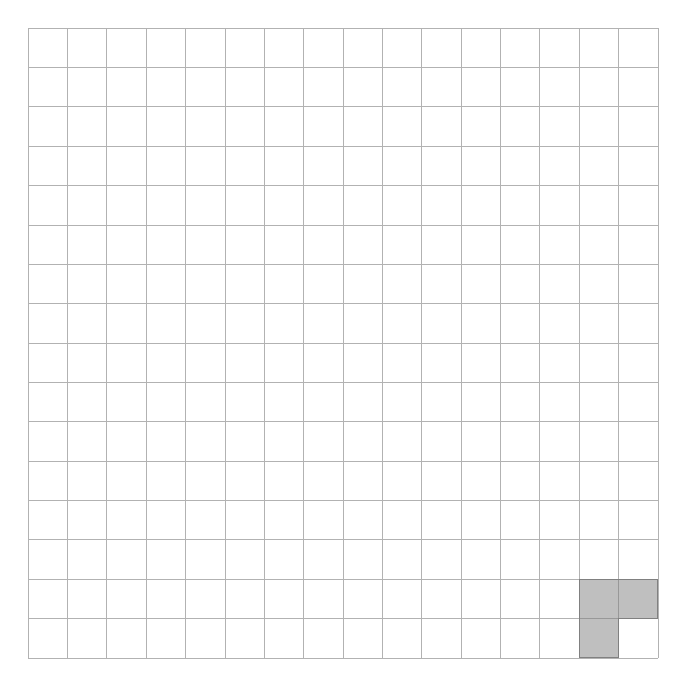
\begin{tikzpicture}[scale=0.5]            
        \draw[help lines, color=black!30] (0,0) grid (16,16);            
        \coordinate (O) at (16,0);
        \tkzDrawPoints[shape=cross out,size=3pt](O);
        \tkzLabelPoints[above](O);
        \pavageL
        \begin{scope}[shift={(-8,8)}]
            \pavageL
        \end{scope}
        \begin{scope}[rotate around={90:(8,0)}]
            \pavageL
        \end{scope}
        \begin{scope}[rotate around={-90:(16,8)}]
            \pavageL
        \end{scope}
        % Les points
        \coordinate (A) at (14,0);
        \coordinate (B) at (15,0);
        \coordinate (C) at (15,1);
        \coordinate (D) at (16,1);
        \coordinate (E) at (16,2);
        \coordinate (F) at (14,2);
        \draw[color=gray,fill=gray,fill opacity=0.5] (A) -- (B) -- (C) -- (D) -- (E) -- (F) -- cycle;
    \end{tikzpicture}

    \begin{enumerate}
        \item Colorier \textbf{en bleu} l'image de la figure grise par l'homothétie de centre $O$ et de rapport $2$.
        \item Colorier \textbf{en rouge} l'image de la figure grise par l'homothétie de centre $O$ et de rapport $4$.
        \item Colorier \textbf{en vert} l'image de la figure grise par l'homothétie de centre $O$ et de rapport $8$.
    \end{enumerate}
\end{exercice*}
\begin{corrige}
    %\setcounter{partie}{0} % Pour s'assurer que le compteur de \partie est à zéro dans les corrigés
    \phantom{rrr}    

    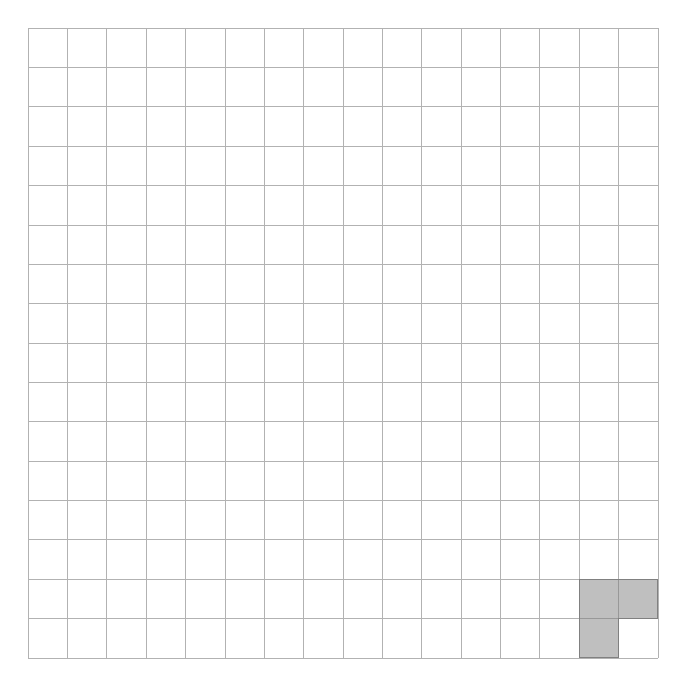
\begin{tikzpicture}[scale=0.5]            
        \draw[help lines, color=black!30] (0,0) grid (16,16);            
        \coordinate (O) at (16,0);
        \tkzDrawPoints[shape=cross out,size=3pt](O);
        \tkzLabelPoints[above](O);
        \pavageL
        \begin{scope}[shift={(-8,8)}]
            \pavageL
        \end{scope}
        \begin{scope}[rotate around={90:(8,0)}]
            \pavageL
        \end{scope}
        \begin{scope}[rotate around={-90:(16,8)}]
            \pavageL
        \end{scope}
        % Les points
        \coordinate (A) at (14,0);
        \coordinate (B) at (15,0);
        \coordinate (C) at (15,1);
        \coordinate (D) at (16,1);
        \coordinate (E) at (16,2);
        \coordinate (F) at (14,2);
        \draw[color=gray,fill=gray,fill opacity=0.5] (A) -- (B) -- (C) -- (D) -- (E) -- (F) -- cycle;
        \imageHomothetyHexaGone{2}{blue};
        \imageHomothetyHexaGone{4}{red};   
        \imageHomothetyHexaGone{8}{mygreen};
    \end{tikzpicture}

    \begin{enumerate}
        \item Colorier \textbf{en bleu} l'image de la figure grise par l'homothétie de centre $O$ et de rapport $2$.
        \item Colorier \textbf{en rouge} l'image de la figure grise par l'homothétie de centre $O$ et de rapport $4$.
        \item Colorier \textbf{en vert} l'image de la figure grise par l'homothétie de centre $O$ et de rapport $8$.
    \end{enumerate}
\end{corrige}

